\documentclass[../../main.tex]{subfiles}
\graphicspath{{../../image/}{../../figure/}}
\begin{document}

\subsection{去噪自编码器}\label{subsection:ch19-去噪自编码器}

我们已经看到了在简单的自编码器中限制潜空间层的维度的重要性，这样能避免模型直接学习恒等映射。\textbf{去噪自编码器}（denoising autoencoder）（Vincent, 2008）也能迫使模型发现数据内部有趣的结构。其背后的思想是用噪声破坏每个输入向量 $x_n$，得到一个修改后的向量 $\widetilde{x}_n$，然后将其输入自编码器，产生输出 $\widehat{x}(x_n,w)$。网络可以通过最小化平方和损失函数来训练，其目的是重建原始的无噪声输入向量：
\begin{align}
E(w)=\frac{1}{2}\sum_{n=1}^{N}\big\|x_n-\widehat{x}(\widetilde{x}_n,w)\big\|^2
\label{align:ch19-denoise}
\end{align}

添加噪声的一种方法是随机地把一些输入变量设置为零。此类输入所占的比例 $v$ 代表噪声水平，并且范围是 $0\le v\le 1$。添加噪声的另一种方法是为每个输入变量添加独立的零均值高斯噪声，其中噪声的规模由高斯分布的方差设定。通过学习去除输入数据中的噪声，网络被迫学习数据方方面面的结构。例如，如果数据包含图像，网络只需要学习到相邻像素值之间的强相关性，就可以纠正被噪声损坏的像素。

更正式地讲，去噪自编码器的训练与\textbf{得分匹配}（score matching）（Vincent, 2011）相关，得分由 $s(x)=\nabla_x\ln p(x)$ 定义。图~\ref{fig:ch19-denoise-manifold} 说明了我们对这种关系的一些直观的理解。自编码器通过学习逆转失真向量 $\widetilde{x}_n-x_n$，学习了数据空间中每个点的一个向量，该向量指向流形，从而指向高数据密度区域。得分向量 $\nabla_x\ln p(x)$ 同样是一个指向高数据密度区域的向量。等到讨论扩散模型时（参见 20.3 节），我们将更深入地探索得分匹配和去噪之间的关系。我们将看到，扩散模型也会学习从那些被噪声破坏的输入中去除噪声。

\begin{figure}[htbp]
\centering
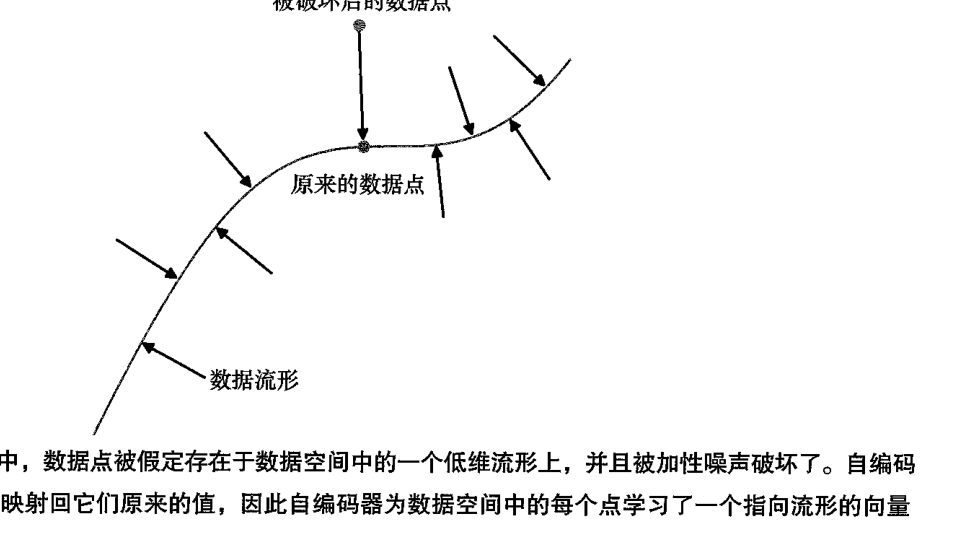
\includegraphics[width=0.8\textwidth]{ch19-fig513-denoise-manifold.png}
\caption{在去噪自编码器中，数据点被假定存在于数据空间中的一个低维流形上，并且被加性噪声破坏了。自编码器会学习将损坏的数据点映射回它们原来的值，因此自编码器为数据空间中的每个点学习了一个指向流形的向量。}
\label{fig:ch19-denoise-manifold}
\end{figure}

\subsection{掩蔽自编码器}\label{subsection:ch19-掩蔽自编码器}

我们已经看到，借助随机遮盖输入子集的自监督学习方式，像 BERT 这样的 Transformer 模型能学习到自然语言的深层次内部表示（参见 12.2 节）。人们很自然地会问，类似的方法能应用于自然图像吗？\textbf{掩蔽自编码器}（masked autoencoder）（He et al., 2021）旨在利用深度神经网络，根据输入图像的损坏版本重建图像，这与去噪自编码器类似。在这种情况下，损坏（corruption）的形式是掩蔽或删除输入图像的一部分。

这种技术通常可以与视觉 Transformer 架构结合起来使用（参见 12.4.1 小节），因为在这种情况下，仅仅通过传递随机选定的输入补丁标记（input patch token）子集给编码器，就可以轻松实现对输入图像的部分进行掩蔽。图~\ref{fig:ch19-mae} 总结了整个算法。

\begin{figure}[htbp]
\centering
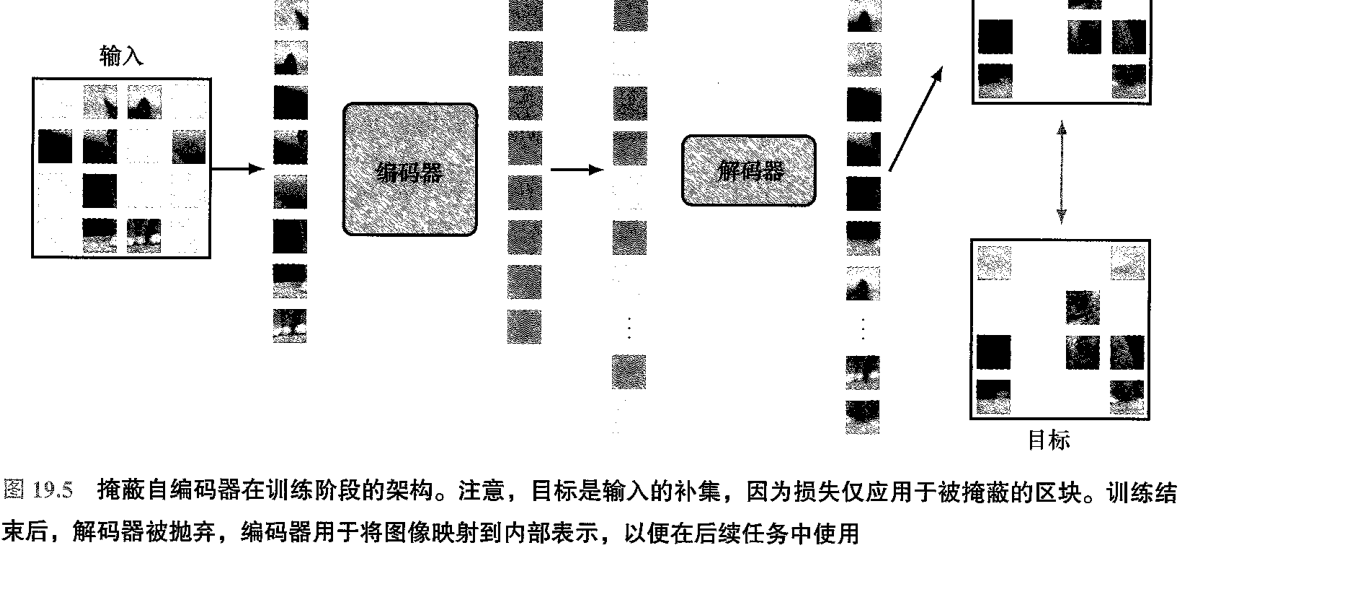
\includegraphics[width=0.85\textwidth]{ch19-fig513-mae.png}
\caption{掩蔽自编码器在训练阶段的架构。注意，目标是输入的补丁，因为损失仅应用于被掩蔽的区块。}
\label{fig:ch19-mae}
\end{figure}

和语言不同，图像具有更多的冗余，并伴有强烈的局部相关性。在一句话中省略一个单词可能会大大增加歧义，然而随机移除图像中的一小块通常对图像的语义影响很小。当输入图像有较高掩蔽比例（通常为 $75\%$）时，算法能学到最佳的内部表示；而 BERT 中的掩蔽比例仅为 $15\%$。在 BERT 中，掩蔽的输入被固定的掩蔽符号替换；而在掩蔽自编码器中，掩蔽的区块简单地被省略。考虑到 Transformer 的计算效率随着输入序列长度的增加而下降，通过省略大量的输入区块，我们可以节省大量的计算资源，因此掩蔽自编码器成为预训练大型 Transformer 编码器的优选。

由于解码器层同样是 Transformer，它需要按照原始图像的维度来运作。因为 Transformer 的输出与输入具有相同的维度，我们需要在编码器输出和解码器输入之间恢复图像的维度。这可以通过重新引入被掩蔽的区块来实现，每个片段标记都增加了位置编码信息，并且由固定的掩蔽标记向量表示。由于解码器表示的维度远高于编码器，解码器 Transformer 拥有的可学习参数远少于编码器 Transformer。解码器的输出对接的是一个可学习的线性层，用于将输出表示映射到像素值空间，而训练损失函数的作用就是简单地对每个图像缺失区块的均方误差取平均值。

图~\ref{fig:ch19-mae-recon} 展示了使用训练成功的掩蔽自编码器重建图像的 $4$ 个例子，展示了训练后的自编码器在生成合理语义上可信的重构能力。然而，我们最终的目标是学习对后续下游任务有用的内部表示，因此我们舍弃了解码器，而把编码器应用于没有遮蔽的完整图像，并配备了一组针对所需应用而微调的新输出层。

\begin{figure}[htbp]
\centering
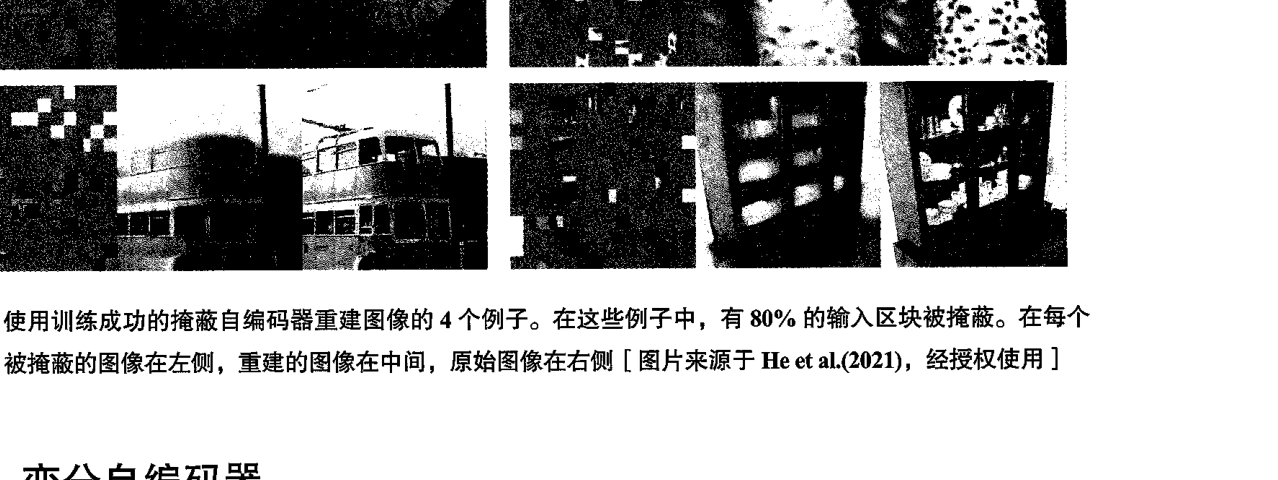
\includegraphics[width=0.9\textwidth]{ch19-fig514-mae-recon.png}
\caption{使用训练成功的掩蔽自编码器重建图像的 $4$ 个例子。在这些例子中，有 $80\%$ 输入区块被掩蔽。在每个例子中，被掩蔽的图像在左侧，重建的图像在中间，原始图像在右侧（He et al., 2021，经授权使用）。}
\label{fig:ch19-mae-recon}
\end{figure}

\end{document}